\documentclass[landscape,10pt]{article}



\usepackage{geometry}
\geometry{
	letterpaper,
	left=5mm,
	right=5mm,
	top=5mm,
	bottom=5mm
}
\usepackage{amsmath,amssymb,tikz}
\usepackage{enumitem,multicol}
\setlength{\columnsep}{2cm}

\pagenumbering{gobble}

\setlength\parindent{0pt}


\begin{document}
	
	\begin{multicols*}{2}
			
		
		\subsection*{Topic 5 - Joint Distributions}
 	
		Car example\\
		
		\begin{tabular}{|c|c|c|c|c|c|}
			\hline
			$ X / Y $ &  0   &  1   &  2   &  3   &  4   \\ \hline
			    0     & 1/2  & 1/16 & 1/32 & 1/32 & 1/32 \\ \hline
			    1     & 1/16 & 1/32 & 1/32 & 1/32 & 1/32 \\ \hline
			    2     & 1/32 & 1/32 & 1/32 & 1/32 & 1/32 \\ \hline
		\end{tabular}
		\\
		
		$ P(X \geq 1, Y \geq 1) = 8/32 $\\
		$ P(X \geq 1) = 6/32 + 5/32 = 11/32 $\\
		$ E(X + Y) =  $\\
		
		
		sample mean: $ \bar{x} = \dfrac{\sum\limits_{i=1}^{n} x_i}{n} $\\
		sample median: middle value if arranged in increasing order\\
		
		
		$ 1^{st} $ quartile $ (Q_1) $ - $ 25^{th} $ percentile\\
		$ 2^{nd} $ quartile $ (Q_2) $ - $ 50^{th} $ percentile\qquad 5 number summary: Min, $ Q_1 $, $ Q_2 $, $ Q_3 $, Max\\
		$ 3^{rd} $ quartile $ (Q_3) $ - $ 75^{th} $ percentile\\
		\\
		\underline{Box Plot}
		

			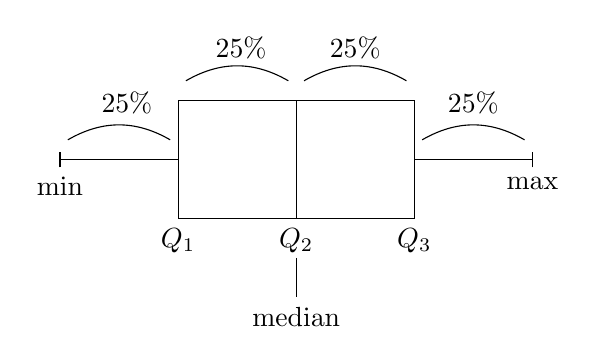
\begin{tikzpicture}[scale=1]
			\draw (-1.5,0.75) -- (0,0.75);
			\draw (-1.5,0.65) -- (-1.5,0.85);
			\node at (-1.5,0.65) [below] {min};
			\draw (0,0) rectangle (3,1.5);
			\node at (0,0) [below] {$Q_1$};
			\draw (1.5,0) -- (1.5,1.5);
			\node at (1.5,0) [below] {$Q_2$};
			\draw (1.5,-0.5) -- (1.5,-1) node[below] {median};
			\node at (3,0) [below] {$Q_3$};
			\draw (3,0.75) -- (4.5,0.75);
			\draw (4.5,0.65) -- (4.5,0.85);
			\node at (4.5,0.65) [below] {max};
			\draw (-1.4,1) to[bend left] (-0.1,1);
			\node at (-0.65,1.2) [above] {$25\%$};
			\draw (0.1,1.75) to[bend left] (1.4,1.75);
			\node at (0.8,1.9) [above] {$25\%$};
			\draw (1.6,1.75) to[bend left] (2.9,1.75);
			\node at (2.25,1.9) [above] {$25\%$};
			\draw (3.1,1) to[bend left] (4.4,1);
			\node at (3.75,1.2) [above] {$25\%$};
			\end{tikzpicture}

		
		
		Measures of spread: IQR $ (Q_3-Q_1) $ and sample variance $ (s^2 \text{ or } \sigma^2) $\\
		$ \sigma^2 = \dfrac{\sum\limits_{i=1}^{n} (x_i - \bar{x})^2}{n-1} $  ,where $ n-1 $ is the degrees of freedom\\
		
		sample standard deviation: $ \sqrt{s^2} $\\
		
		Trimmed mean: take off from both ends and compute new mean. \textit{Example}: Sample of 20. $ 10\% $ trimmed mean $ \to $ take 2 values off from beginning and end so mean of 16 values. Usually to get rid of outliers.\\
		\\
		
 	
		\subsection*{Topic 2}
		
		
		% Definition of circles
		\def\firstcircle{(0,0) circle (1.5cm)}
		\def\secondcircle{(0:2cm) circle (1.5cm)}
		
		\colorlet{circle edge}{blue!50}
		\colorlet{circle area}{blue!20}
		
		\tikzset{filled/.style={fill=circle area, draw=circle edge, thick},
			outline/.style={draw=circle edge, thick}}
		
		\setlength{\parskip}{5mm}
		% Set A and B
		\begin{tikzpicture}[scale=0.5]
		\begin{scope}
		\clip \firstcircle;
		\fill[filled] \secondcircle;
		\end{scope}
		\draw[outline] \firstcircle node {$A$};
		\draw[outline] \secondcircle node {$B$};
		\node[anchor=south] at (current bounding box.north) {$A \cap B$};
		\end{tikzpicture}
		% Set A or B
		\begin{tikzpicture}[scale=0.5]
		\draw[filled] \firstcircle node {$A$}
		\secondcircle node {$B$};
		\node[anchor=south] at (current bounding box.north) {$A \cup B$};
		\end{tikzpicture}
		
		Properties of probability \vspace{-5mm}
		\begin{itemize}
			\item $ P(A \cup B) = P(A) + P(B) - P(A \cap B) $
			\item $ P(A \cap B) = P(A) + P(B) - P(A \cup B) $
			\item $ P(A^c) = 1 - P(A) $
			\item Conditional probability of $ A $ given $ B $: $ P(A|B) = \dfrac{P(A \cap B)}{P(B)} $
			\item $ A $ and $ B $ are independent if $ P(A \cap B) = P(A) P(B) $
		\end{itemize}
 	
		The reliability of a system is the overall probability of success.\\
		$ P(\text{failure}) = 1- P(\text{success}) $

		\begin{center}
			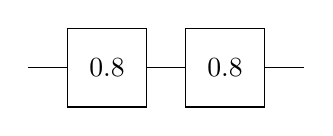
\begin{tikzpicture}
			\draw (-0.5,0.5) -- (0,0.5);
			\draw (0,0) rectangle (1,1);
			\node at (0.5,0.5) {$0.8$};
			\draw (1,0.5) -- (1.5,0.5);
			\draw (1.5,0) rectangle (2.5,1);
			\node at (2,0.5) {$0.8$};
			\draw (2.5,0.5) -- (3,0.5);
			\end{tikzpicture}
		\end{center}	
		\vspace{-10mm}
			\begin{align*}
				P(S) &= P(A \cap B) = P(A) P(B) \\
				 &= 0.8 \cdot 0.8\\
				 &= 0.64
			\end{align*}
		\vspace{-10mm}
		\begin{center}
			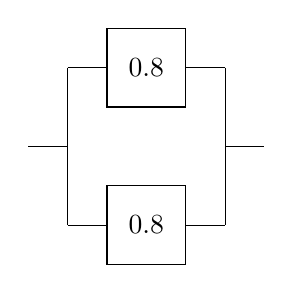
\begin{tikzpicture}
			\draw (0,0) rectangle (1,1);
			\draw (-0.5,0.5) -- (0,0.5);
			\draw (-0.5,0.5) -- (-0.5,-1.5);
			\draw (-1,-0.5) -- (-0.5,-0.5);
			\draw (0,-2) rectangle (1,-1);
			\draw (-0.5,-1.5) -- (0,-1.5);
			\draw (1,0.5) -- (1.5,0.5);
			\draw (1.5,0.5) -- (1.5,-1.5);
			\draw ((1,-1.5) -- (1.5,-1.5);
			\draw (1.5,-0.5) -- (2,-0.5);
			\node at (0.5,0.5) {$0.8$};
			\node at (0.5,-1.5) {$0.8$};
			\end{tikzpicture}
		\end{center}
			\vspace{-10mm}
			\begin{align*}
				P(S) &= P(A \cup B) = P(A) + P(B) - P(A \cap B)\\
				&= 0.8 + 0.8 - 0.64\\
				&= 0.96 
			\end{align*}
	Adding more components to a series system results in loss of reliability, vice versa for parallel systems.

	\newpage
	
	\subsection*{Topic 3}
		
	\textit{discrete random variable} takes on a countable number of values\\
	\textit{probability mass function} (pmf) is a distribution of a discrete random variable $ x $
	\[ f(x) = P(X = x) \]
	requirements for pmf: $ f(x) > 0 $ for all $ x $, and $ \sum\limits_{\text{all } x}^{} f(x) = 1 $\\
	
	\textit{cumulative distribution function} (cdf): $ F(x) = P(X \leq x ) = \sum\limits_{\text{all } t \leq x}^{} f(t) $\\
	
	Bernoulli random variable: Success = $ p $, failure = $ 1- p $\\
	Example:
	\[ SSS = p^3 \qquad SFS = p^2(1-p) \qquad FFS = p(1-p)^2 \qquad FFF = (1-p)^3 \]
	Mean of discrete random variable: $ \mu_x = E(x) = \sum x \cdot p(x) $\\
	$ E(h(x)) = \sum h(x) \cdot f(x) $ is the expected value of $ h(x) $\\
	$ V(x) = \sigma_x^2 = E(x^2) - (E(x))^2 $\\
	
	Binomial Distribution: Bernoulli trials: each trial can result in one or two outcomes (success or fail), trials are independent\\
	Binomial pmf: probability of any outcome sequence from $ n $ Bernoulli trials with $ x $ successes and $ n-x $ fails
	\[ f(x) = P(X=x) = \begin{pmatrix} n\\x \end{pmatrix} p^x (1-p)^{n-x} \]
	Binomial properties: $ E(x) = \mu_x = np $, $ \sigma_x^2 = np(1-p) $\\
	
	Poisson Distribution: number of events occurring in an interval where the expected number of events is proportional to the length of the interval
	\[ f(x) = P(X=x) = \frac{e^{-\lambda} \lambda^x}{x!}, \, \lambda: \text{rate} \]
	Poisson properties: $ E(x) = \lambda $, $ \sigma_x^2 = \lambda $\\
	\\
	\\
	\\
	\\	
	\\
	\\
	\\	
	
	\subsection*{Topic 4}
		
	\textit{Probability Density function} (pdf): A function $ f(x) $ such that for $ a \leq x \leq b $
	\[ P(a \leq x \leq b) = \int_{a}^{b} f(x) \, dx \]	
	cdf of $ X $ is $ F(X) = P(X = x) = \int_{-\infty}^{x} f(t)\,dt $
	
	$ f(x) = F'(x) $\\
	$ P(a \leq x \leq b) = F(b) - F(a) $
	
	Properties of pdf:\\
	$ E(x) = \int_{a}^{b} x \cdot f(x) \, dx $\\
	$ \sigma_x^2 = E(x^2) - (E(x))^2 = \int_{a}^{b} x^2 \cdot f(x) \,dx - \mu_x^2 $\\
	$ E(h(x)) = \int_{a}^{b} h(x) \cdot f(x)\,dx $
	
	If it is a \textit{uniform} distribution, then 
		
		
		
	\end{multicols*}
	
	
	
	
	
	
	
	
	
	
\end{document}